% -*- root: ../Crypto.tex -*-
\section{Hoja 1}
\begin{problem}[1]
	Un general espartano recibe el siguiente mensaje de un amigo de Cantoblanco:

	
	SONFAUHPINPEOCTOHRIANEQLSGCUTUOHEEEQOENRUBSETEIDRELEIT

	¿Qué dice el mensaje?
	
	\solution
	Si consiguiéramos una escítala cuyo diámetro hiciera que entraran 5 letras por fila conseguiríamos el mensaje:

	SUPONGOQUELOHEHECHOBIENPORQUEESDIFICILTENERTANTASUERTE
\end{problem}

\begin{problem}[2]
	Recibes el mensaje VEILRÑW, cifrado usando una clave de Cesar en el alfabeto castellano de 27 letras (con Ñ y W). Lee el mensaje, da las transformaciones para cifrar y descifrar, y cifra el mensaje GRACIAS utilizando la clave correspondiente.

	\solution
	Usando la transformación:
	\[\appl{f_{17}}{ℤ/27}{ℤ/27}\]
	\[f_{17}(x) = x + 17\]

	Se consigue $f_{17}(\{V,E,I,L,R,Ñ,W\}) = \{M,U,Y,B,I,E,N\}$.

	De modo que para cifrar nos basta:
	\[f_{17}^{-1}(x) = f_{-17}(x) = f_{10}(x)\]
	\[f_{10}(\{G,R,A,C,I,A,S\}) = \{P,B,K,M,R,K,C\}\]
\end{problem}

\begin{problem}[3]
	Utilizando el análisis de frecuencias, descifra el siguiente mensaje, del que sabes que está escrito en inglés (26 letras, con W pero sin Ñ) y que ha sido cifrado con una clave de Cesar:
	PXPXKXENVDRUXVTNLXHYMXGMAXYKXJNXGVRFXMAHWGXXWLEHGZXKVBIAXKMXQM

	\solution
	Al hacer el análisis de frecuencias se obtiene:

	\begin{center}
		\begin{tabular}{ l l }
			P & 0.03225806451612903 \\
			X & 0.24193548387096775 \\
			K & 0.06451612903225806 \\
			E & 0.03225806451612903 \\
			N & 0.04838709677419355 \\
			V & 0.06451612903225806 \\
			D & 0.016129032258064516 \\
			R & 0.03225806451612903 \\
			U & 0.016129032258064516 \\
			T & 0.016129032258064516 \\
			L & 0.03225806451612903 \\
			H & 0.04838709677419355 \\
			Y & 0.03225806451612903 \\
			M & 0.08064516129032258 \\
			G & 0.06451612903225806 \\
			A & 0.04838709677419355 \\
			J & 0.016129032258064516 \\
			F & 0.016129032258064516 \\
			W & 0.03225806451612903 \\
			Z & 0.016129032258064516 \\
			B & 0.016129032258064516 \\
			I & 0.016129032258064516 \\
			Q & 0.016129032258064516
		\end{tabular}
	\end{center}

	Se puede ver que la más frecuente entre todas es la letra X. Si tomamos como letra más usada del ingés la E (en vez de la T) se obtiene el mensaje:

	WEWERELUCKYBECAUSEOFTENTHEFREQUENCYMETHODNEEDSLONGERCIPHERTEXT

	Gracias a la transformación $f_{7}(x) = x + 7$.
\end{problem}

\begin{problem}[4]
	La distribución de frecuencias (en porcentaje) en castellano de las 26 letras (es decir, sin W) es aproxi- madamente la siguiente.

	\begin{tabular}{c c c c c c c c c c c c c c c c c c c c c c c c c c c}
		A & B & C & D & E & F & G & H & I & J & K & L & M \\
		12,6 & 1,0 & 5,1 & 5,7 & 13,7 & 0,9 & 0,8 & 0,5 & 7,0 & 0,2 & 0,0 & 4,6 & 3,2 \\
		N & Ñ & O & P & Q & R & S & T & U & V & X & Y & Z \\
		7,0 & 0,1 & 8,8 & 2,9 & 1,1 & 6,6 & 7,2 & 5,1 & 3,9 & 0,8 & 0,1 & 0,6 & 0,3
	\end{tabular}

	Recibes un mensaje escrito en castellano (con ese alfabeto) que ha sido cifrado con el criptosistema de Cesar. Las dos letras más frecuentes en el texto cifrado son, por ese orden, la J y la N. Deduce razonadamente cual puede haber sido la clave utilizada para cifrar.

	\solution
	Lo lógico sería que las letras más frecuentes en el alfabeto se correspondieran con las más correspondientes en el mensaje, de modo que lo primero que a uno se le viene a la cabeza es corresponder la J (la más frecuente en el mensaje) con la E (la más frecuente en el alfabeto). Esto viene a ser la transformación $f_{-5}=f_{21}$, la cual manda la N (la segunda más frecuente en el mensaje) a la I (que no es la segunda más frecuente en el español).

	De modo que igual la segunda más frecuente en el mensaje es la que se corresponde con la más frecuente en el alfabeto ($f_{-9}=f_{17}$). Con esta transformación se consigue:
	\[f_{17}(J)=A\]
	\[f_{17}(N)=E\]
	Lo cual es más coherente, ya que hace una correspondencia entre las 2 letras más frecuentes del alfabeto (la E y la A) con las 2 más frecuentes del mensaje.
\end{problem}

\begin{problem}[5]
	Interceptamos un mensaje en el que dos profesores hablan de las asignaturas del plan de estudios de Matemáticas. El mensaje es el siguiente:

	DONQONHOSDGXQKCHDKSNSJSDOQOBDCUQ

	Sabemos que el mensaje ha sido cifrado utilizando una sustitución simple en el alfabeto castellano de 27 letras (con Ñ y W), y sospechamos que en el mensaje original aparecía la palabra CALCULO. Lee el mensaje.

	\solution
	Haciendo el análisis de frecuencias del mensaje interceptado se obtiene:

	\begin{center}
		\begin{tabular}{l l}
			D & 0.15625 \\
			O & 0.15625 \\
			N & 0.09375 \\
			Q & 0.125 \\
			H & 0.0625 \\
			S & 0.125 \\
			G & 0.03125 \\
			X & 0.03125 \\
			K & 0.0625 \\
			C & 0.0625 \\
			J & 0.03125 \\
			B & 0.03125 \\
			U & 0.03125
		\end{tabular}
	\end{center}

	Dentro del mensaje interceptado CALCULO se corresponde con NQONHOS, para darse cuenta basta con fijarse que hayan dos pares de letras iguales al igual que pasa en CALCULO. Con dicha correspondencia de letras tenemos (mostramos el mensaje cortado en 2, donde la fila de debajo de cada trozo se corresponde con lo que llevamos descifrado):

	\begin{center}
		\begin{tabular}{c c c c c c c c c c c c c c c c}
			D & O & N & Q & O & N & H & O & S & D & G & X & Q & K & C & H \\
			\_ & L & C & A & L & C & U & L & O & \_ & \_ & \_ & A & \_ & \_ & U
		\end{tabular}
	\end{center}

	\begin{center}
		\begin{tabular}{c c c c c c c c c c c c c c c c}
			D & K & S & N & S & J & S & D & O & Q & O & B & D & C & U & Q \\
			\_ & \_ & O & \_ & O & \_ & O & \_ & L & A & L & \_ & \_ & \_ & \_ & A
		\end{tabular}
	\end{center}

	Puesto que el análisis de frecuencias nos dice que la D es la letra que más aparece, probaremos a corresponderla con la letra E:

	\begin{center}
		\begin{tabular}{c c c c c c c c c c c c c c c c}
			D & O & N & Q & O & N & H & O & S & D & G & X & Q & K & C & H \\
			E & L & C & A & L & C & U & L & O & E & \_ & \_ & A & \_ & \_ & U
		\end{tabular}
	\end{center}

	\begin{center}
		\begin{tabular}{c c c c c c c c c c c c c c c c}
			D & K & S & N & S & J & S & D & O & Q & O & B & D & C & U & Q \\
			E & \_ & O & \_ & O & \_ & O & E & L & A & L & \_ & E & \_ & \_ & A
		\end{tabular}
	\end{center}

	Fijándonos en que la K y la C son las siguientes letras con mayor frecuencia, y que de entre las no utilizadas del alfabeto, la S y N son las siguientes que tienen más frecuencia en español. Probando se llega a que la K va a la N, y la C a la B.

	\begin{center}
		\begin{tabular}{c c c c c c c c c c c c c c c c}
			D & O & N & Q & O & N & H & O & S & D & G & X & Q & K & C & H \\
			E & L & C & A & L & C & U & L & O & E & \_ & \_ & A & N & B & U
		\end{tabular}
	\end{center}

	\begin{center}
		\begin{tabular}{c c c c c c c c c c c c c c c c}
			D & K & S & N & S & J & S & D & O & Q & O & B & D & C & U & Q \\
			E & N & O & \_ & O & \_ & O & E & L & A & L & \_ & E & B & \_ & A
		\end{tabular}
	\end{center}

	Llegados a este punto, somos capaces de adivinar que lo que pone el mensaje es:

	EL CALCULO ES TAN BUENO COMO EL ALGEBRA
\end{problem}


\begin{problem}[6]
	Interceptamos cuatro mensajes cifrados. Sabemos que tanto los mensajes en claro como los mensajes cifrados han sido escritos utilizando el alfabeto ingléss de 26 letras. Las frecuencias con que cada letra aparece en cada mensaje son las siguientes:

	\begin{center}
		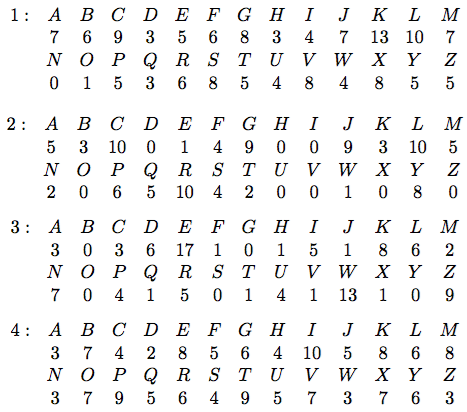
\includegraphics[width=0.5\textwidth]{img/freqsEj1_6}
	\end{center}

	\solution
	
\end{problem}
